\documentclass{article}%
\usepackage[T1]{fontenc}%
\usepackage[utf8]{inputenc}%
\usepackage{lmodern}%
\usepackage{textcomp}%
\usepackage{lastpage}%
\usepackage{geometry}%
\usepackage{float}%
\usepackage{biblatex}%
\usepackage{hyperref}%

\addbibresource{citations.bib}
\geometry{tmargin=1cm,lmargin=0.75cm,rmargin=0.75cm}%
\usepackage{graphicx}%
\setlength{\parskip}{0.2em}%
%
\title{Determination of the Compton wavelength, $\lambda_0$ through experimental investigation the Compton effect.}%

\author{Brian Rogers}

\date{}%
%
\begin{document}%
\maketitle
\section*{Abstract}
This experiment seeks investigate the Compton effect and subsequently, to measure the Compton wavelength, $\lambda_0$ during examination of the Compton effect. Using two materials, plexiglass and aluminium were used to estimate $\lambda_0 = (2.39 \pm 0.17) \times 10^{-12}$ m. 
\section{Introduction}
\subsection{Historical background}
Compton scattering is the process in which a high energy photon collides inelastically with a charged particle. Energy is imparted on the charged particle with the measurable effect of a decrease in the photon's wavelength.
This idea was presented by Arthur Compton in 1923 \cite{Compton} to which he received half of the Nobel prize four years later "for his discovery of the effect named after him". \cite{Nobel}
\subsection{Theory}

\begin{figure}[H]
    \centering%
    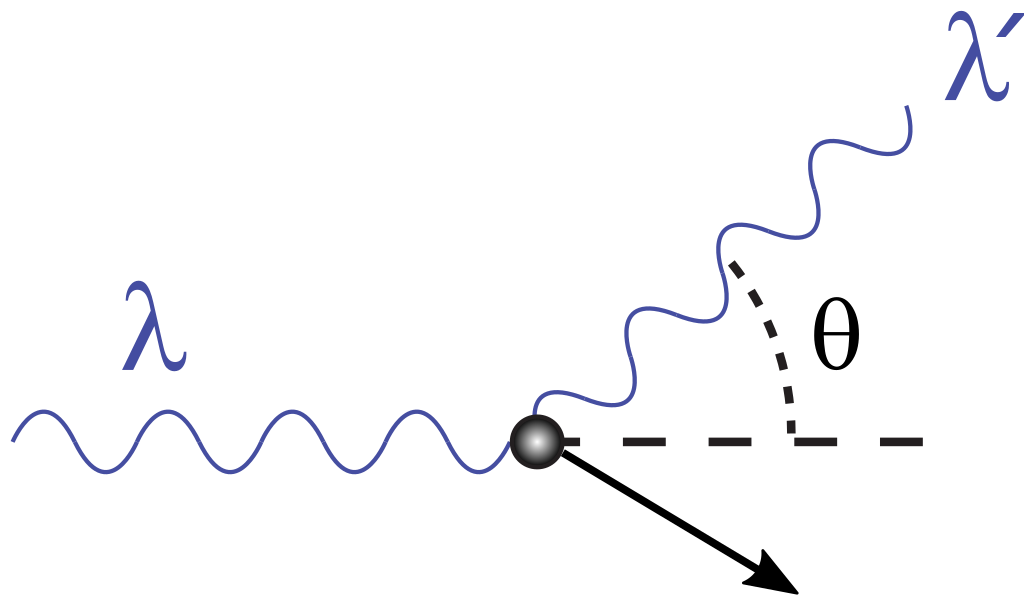
\includegraphics[width=150px]{compton_scattering_diagram.png}
    \caption{Schematic diagram of a photon of wavelength, $\lambda$ scattering at an angle $\theta$ after colliding with an electron. After the collision the photon has reduced wavelength of $\lambda^{\prime}$ \cite{Diagram}}%
\end{figure}
By considering the conservation of momentum it is possible to derive that 

\begin{equation}
    \rho_{\lambda}^2 - 2\rho_{\lambda}\rho_{\lambda^\prime}cos(\theta) + \rho_{\lambda^\prime}^2 = \rho_{e}^2
\end{equation}

By considering the energy of the system we can also state
\begin{equation}
    \frac{K^2}{c^2} + 2Km_0 = p_e^2 
\end{equation}
where $K = c(p_0 - p_1)$

Equating both conservation statements we can say
\begin{equation}
   m_0c(p_0 - p_1) = p_0p_1(1- cos(\theta))
\end{equation}
and so
\begin{equation}
    \frac{1}{p_1} - \frac{1}{p_0} = \frac{1}{m_0c} (1 - cos(\theta))
\end{equation}
Multiplying by Planck's constant and using the Einstein-DeBroglie relation for wavelength and momentum it possible to describe figure 1 mathematically as 

\begin{equation}
    \Delta \lambda = \lambda^\prime - \lambda = \frac{h}{m_0c} (1 - cos(\theta))
\end{equation}
where the Compton wavelength is $\lambda_0 =  \frac{h}{m_0c}$
\section{Methodology}
The experimental setup is shown in the following diagram.  
\begin{figure}[H]
    \centering%
    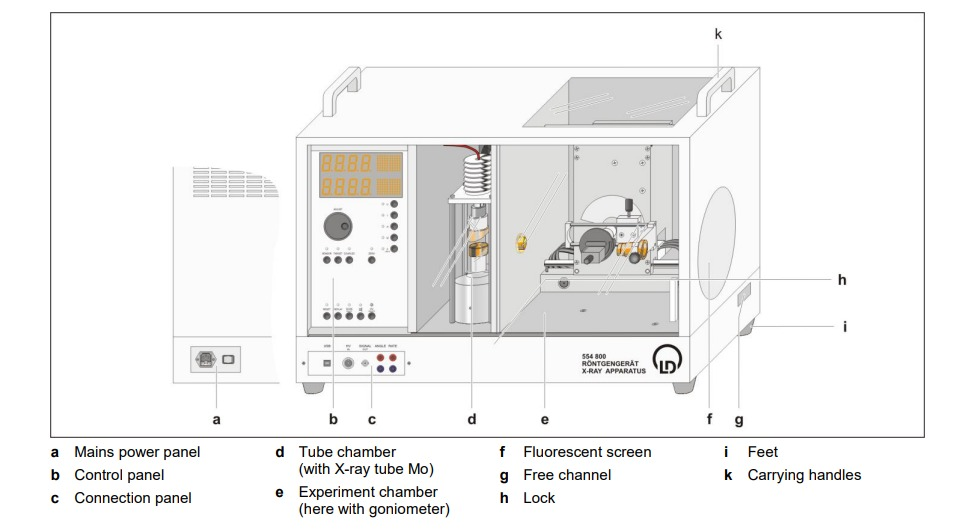
\includegraphics[width=400px]{setup.jpeg}
    \caption{Experimental setup. The detector is coneected to computer with "CASSY 2" software for data recording and analysis.}%
\end{figure}

By introducing a detector into the experiment chamber ("e") attached to the CASSY 2 software, it is possible to record photon counts at different "channels" of energies. Furthermore, we can vary the scattering angle by either changing the detector angle, the angle of the target or a combination of both using the control panel ("b"). 
\section{Results}
\subsection{Plexiglass}
Using the CASSY 2 software the following graph can be plotted describing the distribution of photon counts within energy channels.

\begin{figure}[H]
    \centering%
    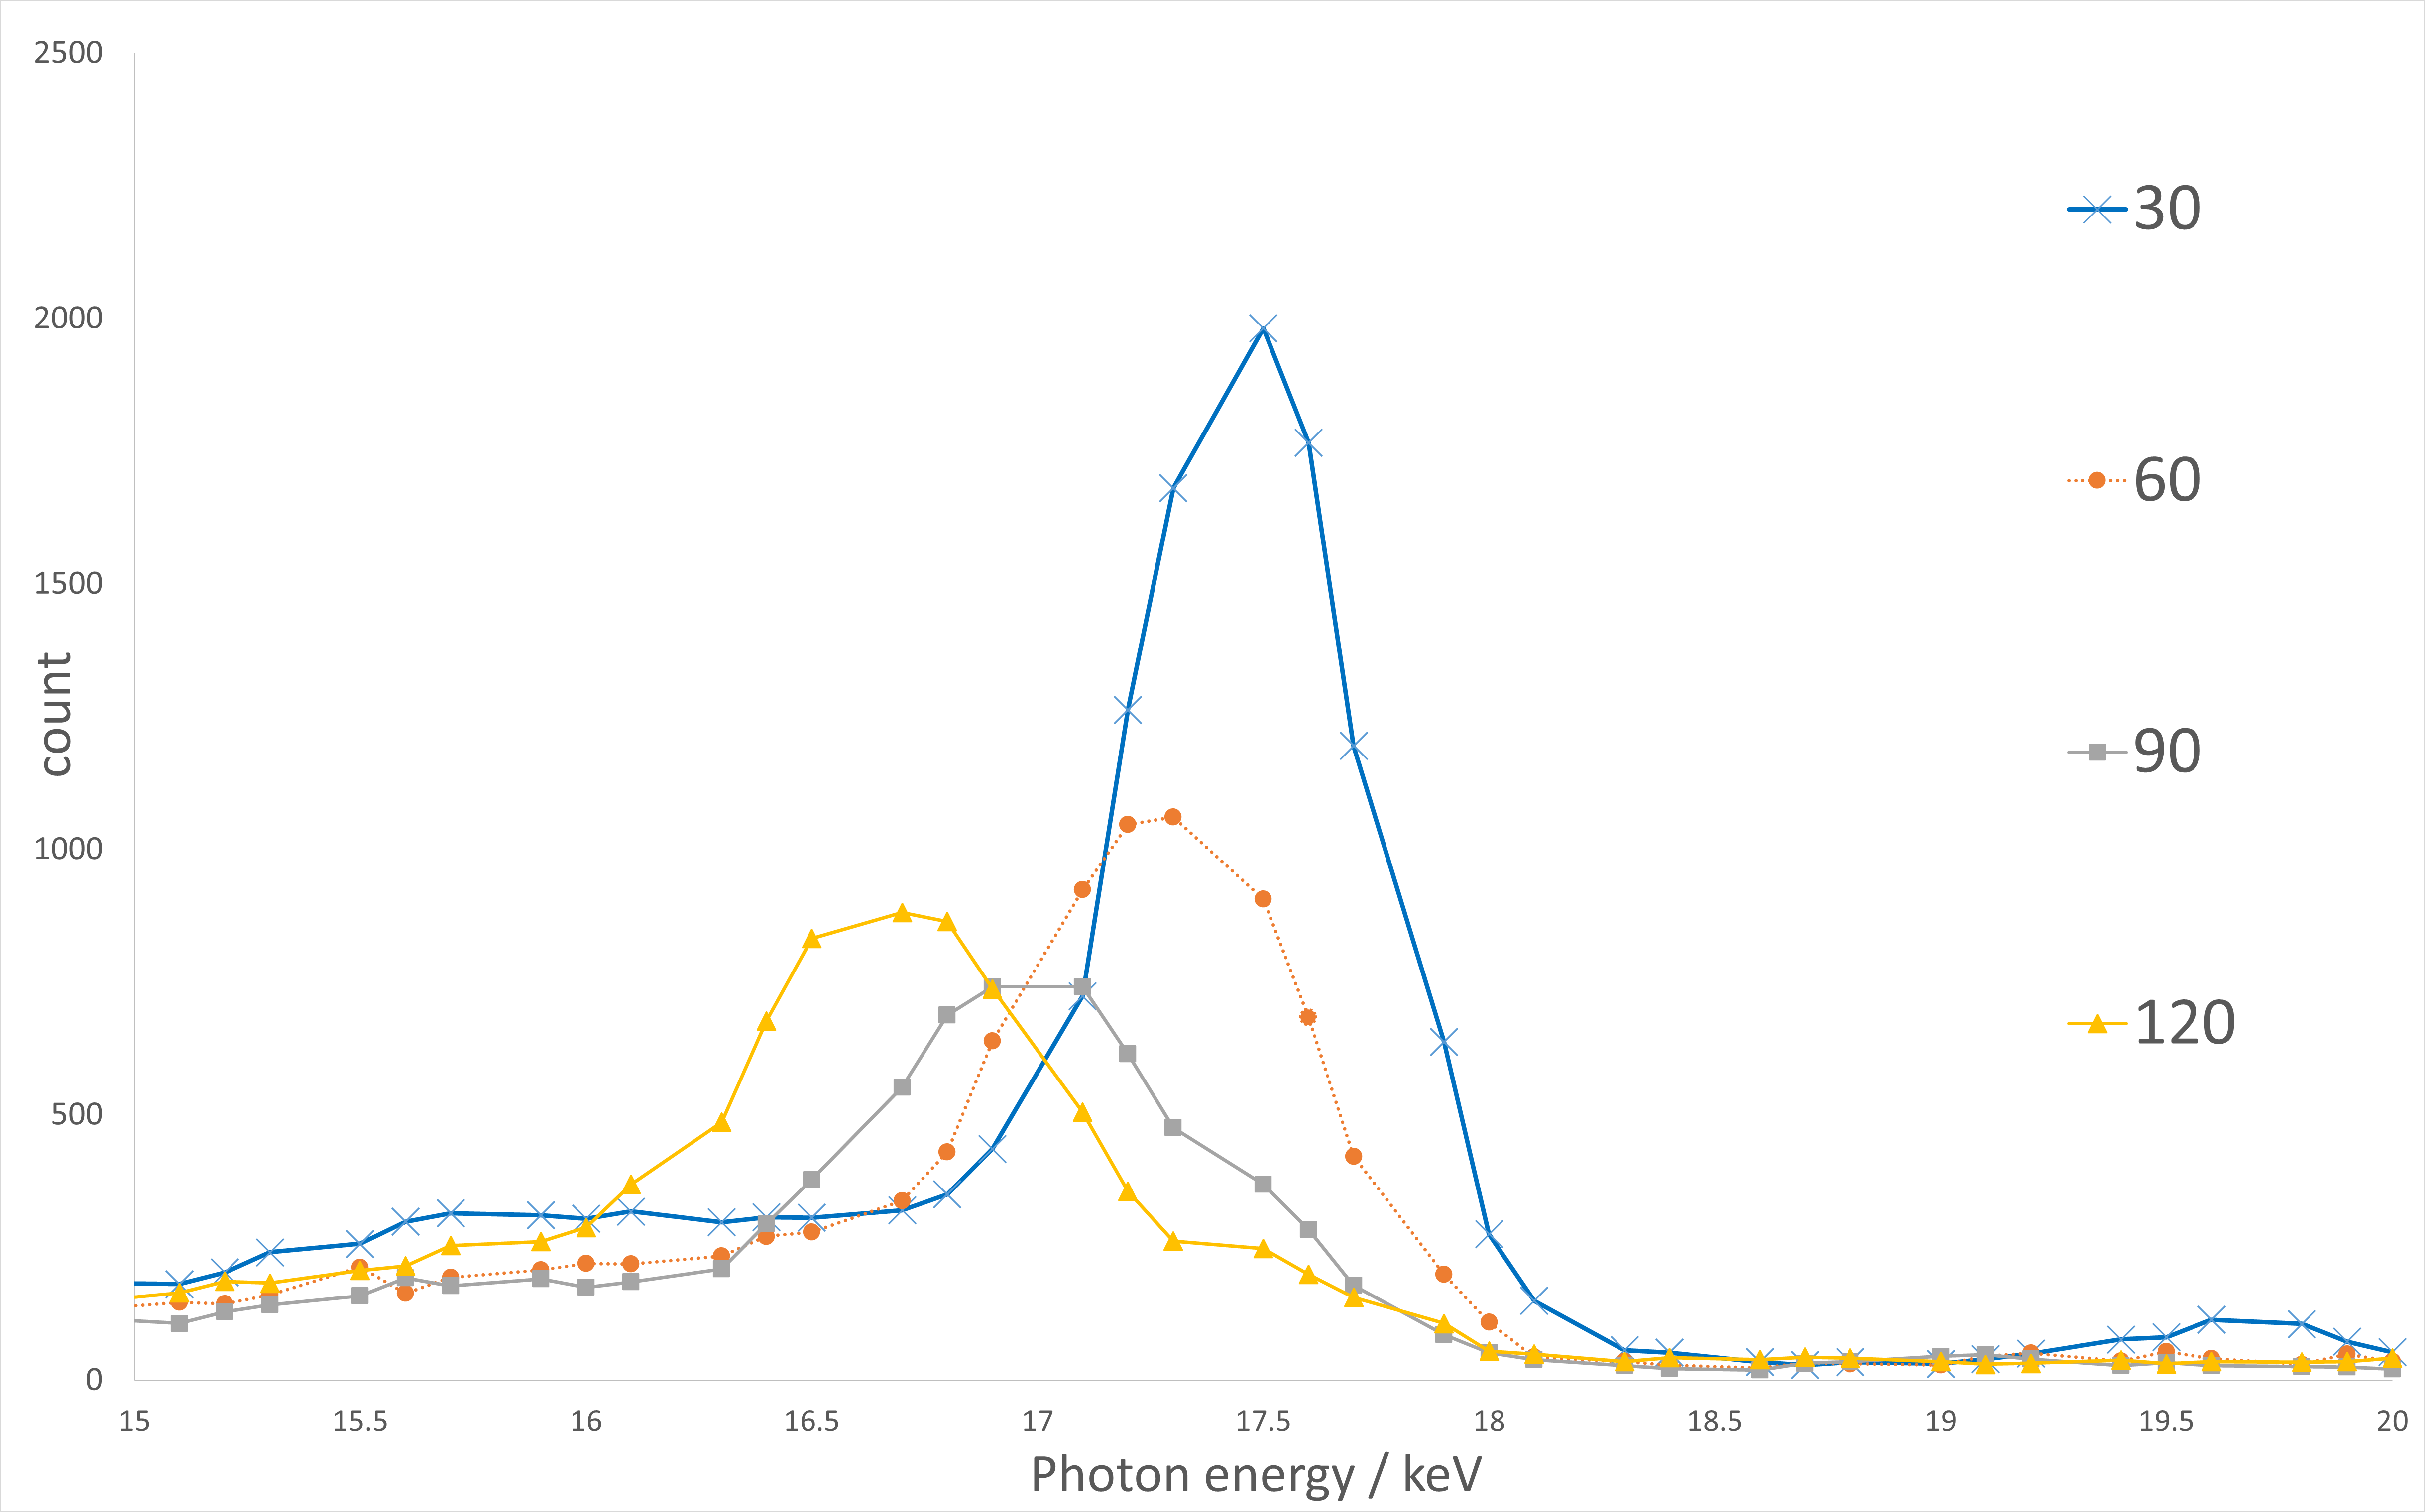
\includegraphics[width=400px]{plexi_plot.png}
    \caption{Plot of count versus phton energy recorded by the detector and processed by the CASSY 2 software.}%
\end{figure}

From this graph it is evident that the as the scattering angle increases, the peak photon energy decreases. By comparing the peak values to a the accepted value of the unshifted peak value of our source $E=17.44 keV$ we can then calculate the change in photon energy between the peaks and hence the change in wavelength of the scattered photon.
This was not possible for the second experiment were the secondary (reflected) peak was used as a reference for the unshifted wavelength. The software seemed to flucuate between primary peak values but with relative consideration to the distance between the primary and secondary peak, the expected trend emerged.
This has implications for the relability of both sets of measurements.

A summary of the measurements recorded for the plexiglass target are the following:
\begin{table}[H]
    \begin{centering}
    \begin{tabular}{|p{3cm}|p{3cm}|p{3cm}|p{3cm}|} 
        \hline
        Angle / $^\circ$ & $\Delta \lambda$ / pm & $\sigma_{\lambda}$ / pm  \\ [0.75ex] 
        \hline\hline
        60 & 0.82 & 0.31 \\ 
        \hline
        90 & 1.66 & 0.42 \\
        \hline
        120 & 3.40 & 0.33 \\
        \hline
        130 & 3.40 & 0.22 \\
        \hline
    \end{tabular}
    \caption{Results from the plexiglass target across detection angles. $\Delta \lambda$ is calculated from a fixed reference energy peak of $E=17.44keV$.}
    \end{centering} 
\end{table}
\subsection{Aluminium}
A similiar process is followed for the aluminium target. However, in this instance aluminium has two peaks. The righter, less intense peak is the photons that I assume to be "elastically" scattered by the target. The more intense peak is formed by photons that have been inelastically scattered as outlined by the Compton model.
\begin{figure}[H]
    \centering%
    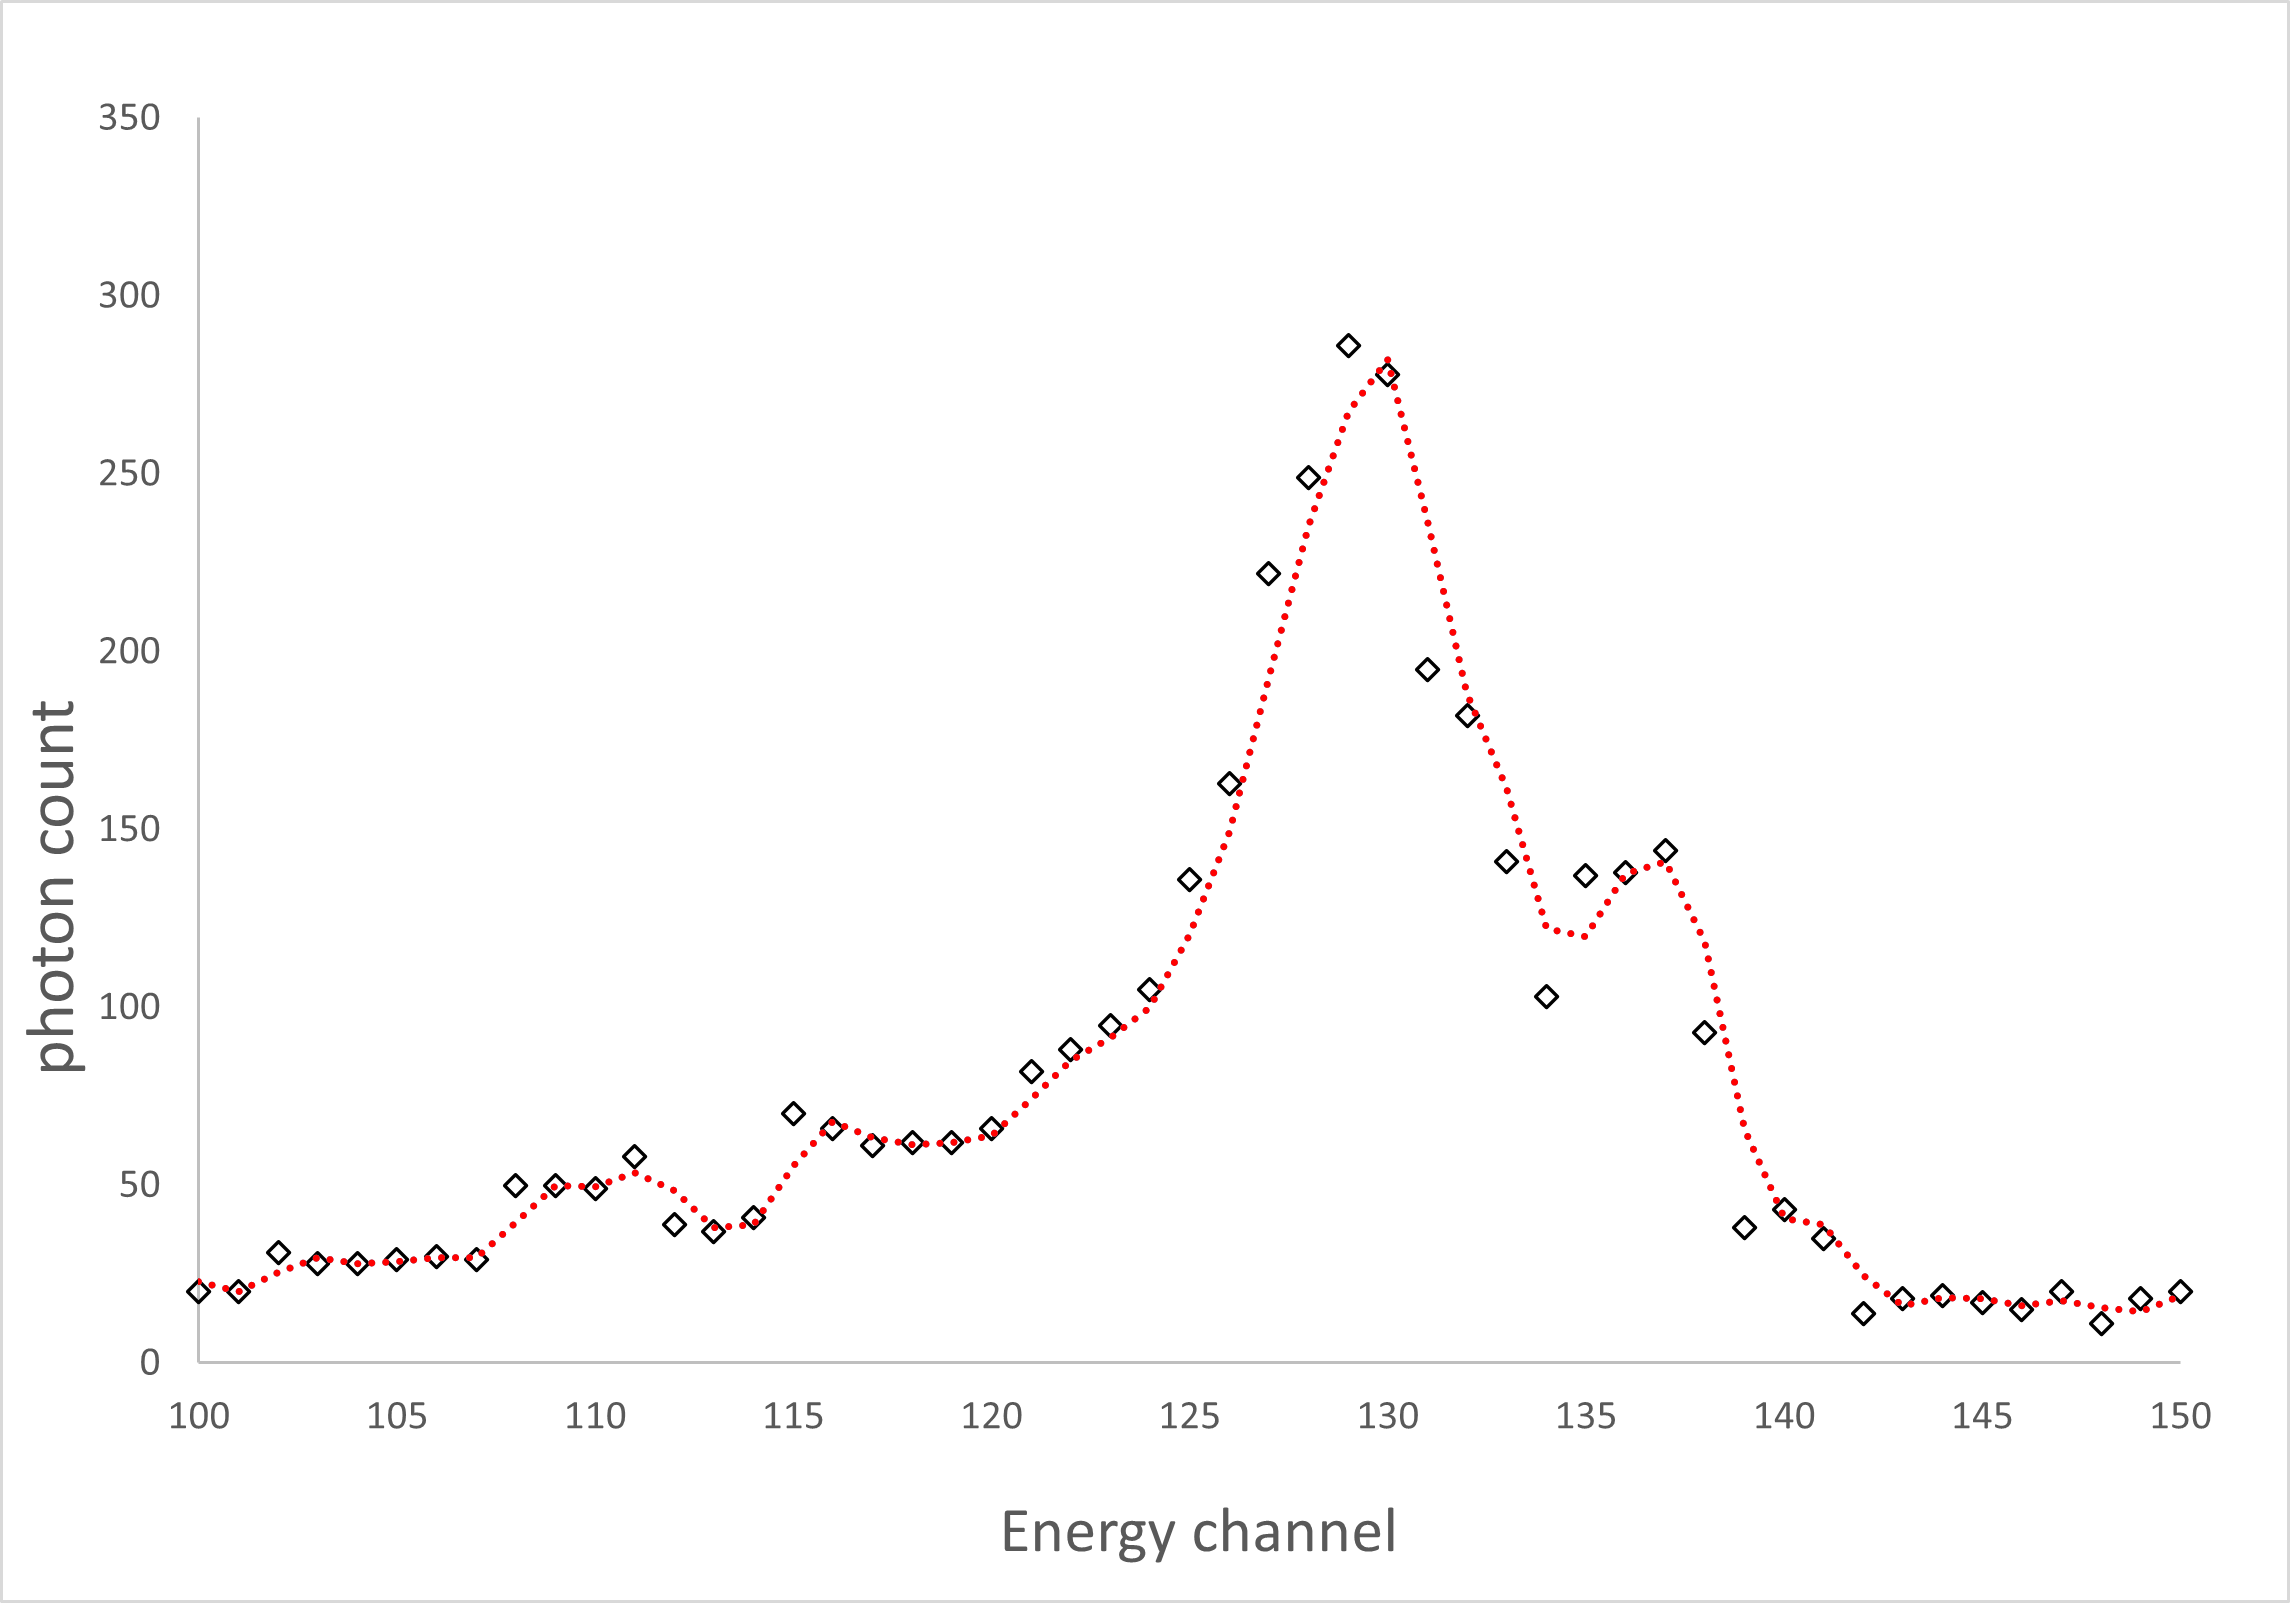
\includegraphics[width=400px]{al_plot.png}
    \caption{Plot of count versus phton energy recorded for the Al target at inclination $30^\circ$.}%
\end{figure}
Measurements for the aluminium target are summarised in the following table.
\begin{table}[H]
    \begin{centering}
    \begin{tabular}{|p{3cm}|p{3cm}|p{3cm}|p{3cm}|} 
        \hline
        Angle / $^\circ$ & $\Delta \lambda$ / pm & $\sigma_{\lambda}$ / pm  \\ [0.75ex] 
        \hline\hline
        30 & 4.71 & 0.55 \\ 
        \hline
        35 & 3.94 & 0.56 \\
        \hline
        40 & 2.58 & 0.54 \\
        \hline

    \end{tabular}
    \caption{Results from the aluminium target across angles of target inclination. Scattering angles are adjusted for future calculations. $\Delta \lambda$ is calculated from a the difference between the peaks of the doublet recorded by the CCD. }
    \end{centering} 
\end{table}
\subsection{Measurement of error}
The possibility of repeat measurements were limited by the exposure time required to gain appreciable photon count rate. With greater time to perform experiments, I would have repeated at each angle taking the standard deviation of the peak energy as a better estimation of the error.

Instead, making the assumption that the count rate followed a Poisson distribution and that the error in this count at the peak, N could be given as
   
\begin{equation}
    \sigma_{E} = \sqrt{N}
\end{equation}

It follows that one standard deviation or the error corresponds to energy values that deviate $\pm \sigma_{E}$ from this peak. We can convert this error into the error in the wavelength by calculating the upper and lower bounds on each peak value.
This means the range of values of the peak width will fall between the difference of the maximum and minimum values of each peak respectively. 


\section{Analysis}

\subsection{Plexiglass}

From the summary presented in table 1, if we take each data point to be an independent measurement of $\lambda_0(i)$, we can take a weighted mean as follows

\begin{equation}
    \overline{\lambda_0} = \frac{\sum{w_i\lambda_0(i)}}{\sum{w_i}}
\end{equation}

were $w_i$ is the weight of the measurement given in terms of it's error, $\sigma_{\lambda}$ as 

\begin{equation}
    w_i = \frac{1}{\sigma_{\lambda}^2}
\end{equation}

The overall error in the can be estimated as the standard deviation across n measurements,

\begin{equation}
    \sigma_{\lambda} = \sqrt{\frac{\sum{(\lambda_0 - \overline{\lambda_0})^2}}{n - 1}}
\end{equation}



We can then determine that $\lambda_0 = (2.32 \pm 0.14) \times 10^{-12}$ m. This values lies within one standard error of the literature value of $\lambda_0 = 2.43 \times 10^{-12}$ m \cite{NIST}. We can then claim this measurement is in "excellent agreement" \cite{HH} with the literature.
The results shown in table 1 were plotted in the following graph with error bars determined from above. 

\begin{figure}[H]
    \centering%
    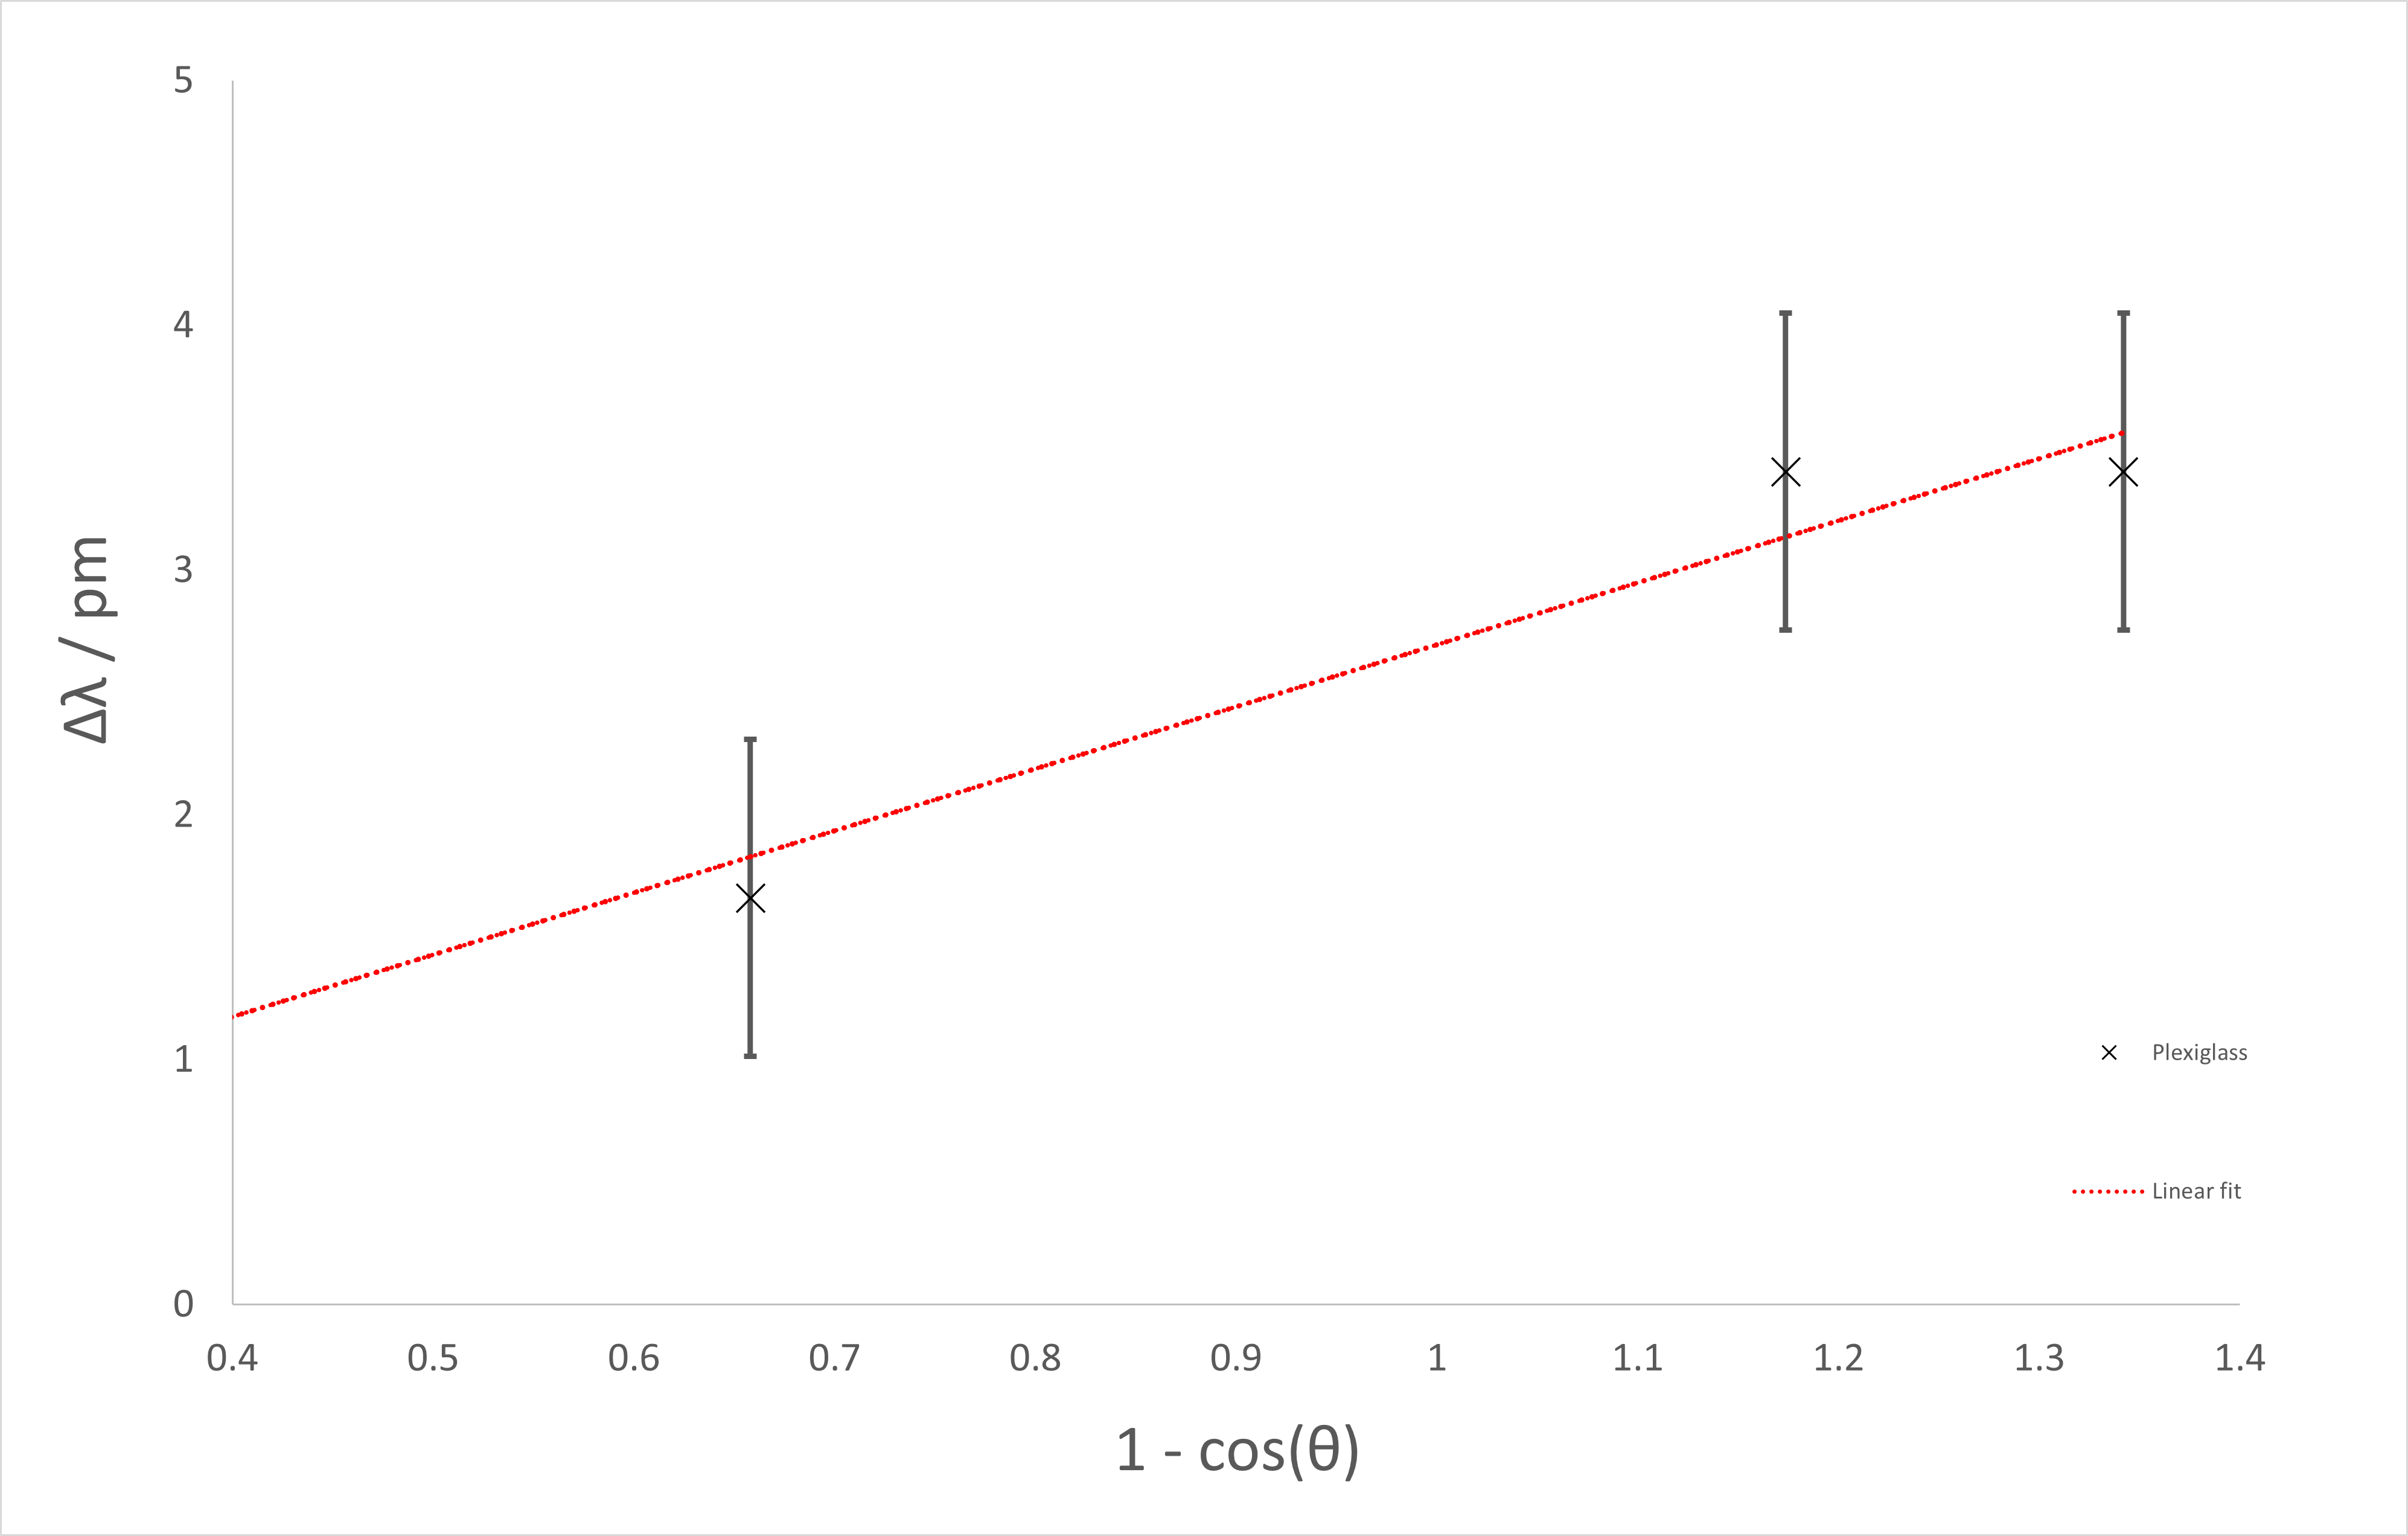
\includegraphics[width=400px]{plexi_graph.png}
    \caption{Plot of $\Delta \lambda$ on $1 - cos(\theta)$.}%
\end{figure}


\subsection{Aluminium}
Using a simliar process as above for the aluminium sample, the Compton wavelength can be calculated as $\lambda_0 = (2.61 \pm 0.41) \times 10^{-12}$ m.

A plot of the analysis can be shown below.
\begin{figure}[H]
    \centering%
    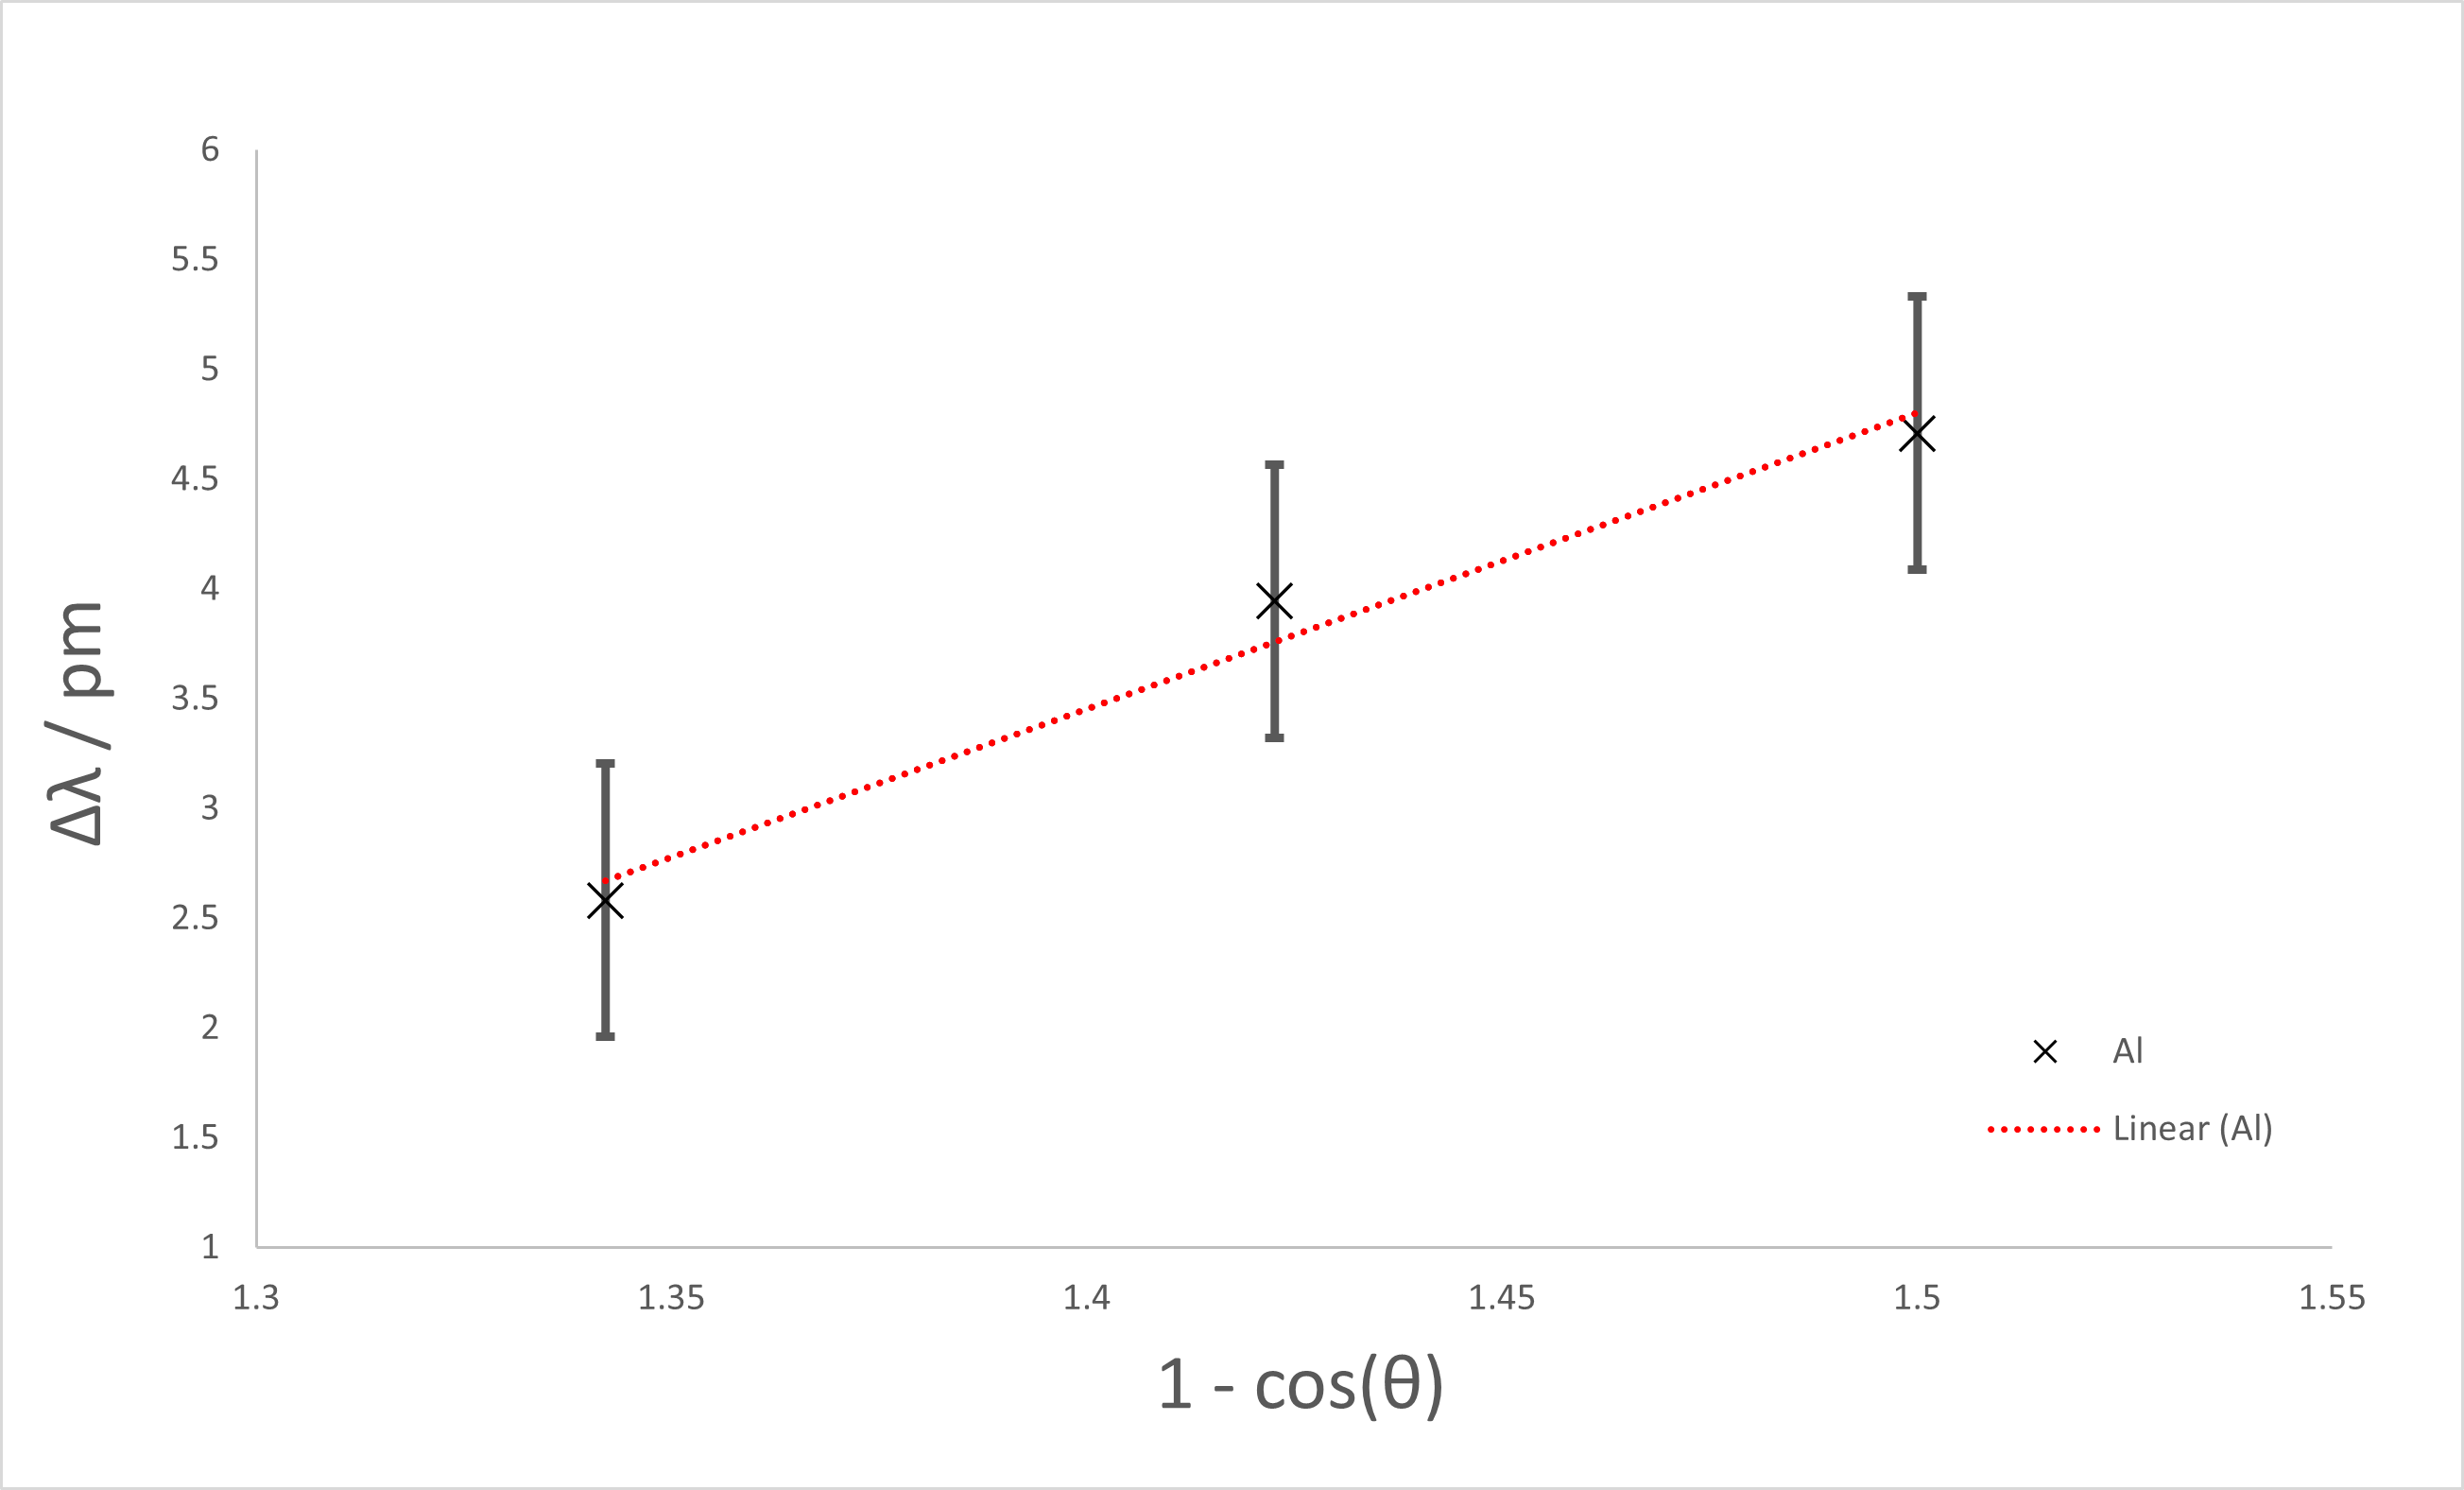
\includegraphics[width=400px]{Al_graph.png}
    \caption{Plot of $\Delta \lambda$ on $1 - cos(\theta)$.}%
\end{figure}

The measurement of the Compton wavelength is within one standard error ($\sigma_{\lambda}$) of the literature value. \cite{NIST} Therefore, we have "excellent agreement" with the literature. \cite{HH}
This measurement is less precise than the plexiglass measurement primarily due to the decrease in count rate and therefore an increase in error as outlined with the Poission estimate for error in equation (6). The overestimate of the value for the Compton wavelength may be a result of the increased variance associated with the lower count values.
By increasing the exposure time or measuring less extreme scattering angles it may be possible to increase the detection rate and increase our precision of measurement.
\subsection{Estimation of the Compton wavelength, $\lambda_0$.}%
Combining both measurements of the Compton wavelength using a weighted mean and estimating the error as the standard deviation of these measurements yields 
$\lambda_0 = (2.39 \pm 0.17) \times 10^{-12}$ m. Although this value agrees with the consenus measurement, it provides a slight underestimation. This may be a function of a lack of data points in both sections of the experiment. Additionally, various other materials could be used to discern if our choice of materials has an effect on our measurement.

\section{Conclusion}
I have investigated and provided evidence that supports the Compton effect. I have measured the Compton wavelength to be $\lambda_0 = (2.39 \pm 0.17) \times 10^{-12}$ m, a value which align with the current values in the literature. I have also described some errors in my experimental method that can be improved upon for future investigations.
\printbibliography
\end{document}